\documentclass{article}

\usepackage[utf8]{inputenc}
\usepackage{amsfonts}
\usepackage{amsmath}
\usepackage{amsthm}
\usepackage{amssymb}
\usepackage{graphicx}
\usepackage{bbm}
\usepackage{wrapfig}
\usepackage{hyperref}
\usepackage[dvipsnames]{xcolor}

\newtheorem{theorem}{Theorem}
\newtheorem{proposition}{Proposition}


\usepackage{geometry}
\geometry{
	letterpaper,
	left=0.57in,
	right=0.57in,
	top=0.76in,
	bottom=0.76in,
}

\newcommand{\tcb}{\textcolor{blue}}



\title{Data market draft}


\begin{document}

\maketitle

\section{Introduction}
In this draft, I first give an overview of high-level questions, then detail them in a closer look, using a simple peer-to-peer two-stage electricity market formulation. Main question that we want to tackle is \emph{how to couple data market and peer-to-peer electricity market?} What appears to be a starting point is to decide, what is the information being sold on the data market and what are the incentives for the agents (prosumers) to purchase it. The idea might be to give the agents an access to the forecasts of the other agents, so that they can improve their own forecasts. Based on these forecasts, each agent makes a decision on the first stage such that the balancing costs on the second stage are minimized. 

\begin{itemize}
    \item Who sells the forecasts? Do forecasts sellers participate in electricity market too? What is the motivation for the agents to sell their forecasts and how the forecasts impact the costs of the agents?
    %We can consider a situation, in which e.g. wind-farm, which might have better knowledge about its future generation might want to sell the forecasts based on this knowledge
    
    \item What should be forecast pricing in these models? If it is based on the utility improvement, then what information is necessary to be available for the market operator/sellers to evaluate it? 
    \begin{itemize}
        \item What information do forecast buyers report besides their base forecast?
        
        \item How to make this mechanism truthful?
        
        \item How to evaluate the impact of the forecast? 
    \end{itemize}
    
    \item Is it relevant to consider the dynamics of the forecast market (i.e., reputation-based effect)?
\end{itemize}

We next consider these questions in more details in the setting of a peer-to-peer electricity market.

\subsection{Peer-to-peer market}
We consider a framework with several buyers (of the forecasts) who also participate in the electricity market. We employ a two-stage electricity market design consisting of day-ahead and balancing (real-time) markets. We assume the presence of a backup retailer from whom the community can purchase energy both in day-ahead (hereafter, referred to as first stage) and in real-time (hereafter, referred to as second stage). Therefore, we fix the buying (b) and selling (s) prices for first (or day-ahead $p_{da}$) and second (or real time $p_{rt}$) stages, such that $p^b_{rt} > p^{b}_{da} > p^{s}_{da} > p^s_{rt}$.

We denote the trade between agent $i$ and $j$ as $q_{ij}$ and impose a bilateral trading reciprocity constraint $q_{ij} + q_{ji} = 0$. Denote $d_i$ as agent $i$'s demand and $\Delta g_i$ as agent $i$'s renewable energy generation (wind, solar, ...), which we assume to be a random variable. Then, each agent has to make a trading decision in the first stage (day-ahead market) about acquiring ($q^{da,b}_i$) or selling ($q^{da,s}_i$) energy at prices $p^{b}_{da}$, $p^{s}_{da}$ respectively. At the second stage (real-time market), agents settle imbalances after observing the realization of $\Delta g_i$ for the prices $p^{b}_{rt}$ (buying) and $p^{s}_{rt}$ (selling). 

\begin{equation}\label{eq: two-stage initial formulation}
    \begin{aligned}
        \min_{q^{da}_i, q^{rt}_i, \mathbf{q}_{i}} \quad &  \overbrace{p^b_{da} q^{da,b}_i - p^s_{da} q^{da,s}_i}^{1^{st} \text{ stage costs }} + \mathbb{E}\Big[\,\overbrace{p^b_{rt} q^{rt, b}_i - p^s_{rt} q^{rt,s}_i}^{2^{nd} \text{ stage costs }} \,\Big] \\
        s.t. \quad & q^{da,b}_i \geq 0, q^{da,s}_i \geq 0, q^{rt,b}_i \geq 0, q^{rt,s}_i \geq 0\\
        & q_{ij} + q_{ji} = 0, \qquad \forall j \in \Gamma_i\\
        & q_{ij} \leq \kappa_{ij}, \qquad \forall j \in \Gamma_i \\
        & d_i = \Delta g_i + \sum_{j \in \Gamma_i} q_{ij} + q^{da,b}_i - q^{da,s}_i + q^{rt,b}_i - q^{rt,s}_i\\
    \end{aligned}
\end{equation}

An additional and important question is to determine when the inter-agent electricity trading is taking place, i.e., on the day-ahead or on the real-time market. If everything was known in advance (i.e., $\Delta g_i$ is deterministic), then the two formulations coincide. Introducing stochasticity to the model poses several questions regarding the organization of the peer-to-peer market and on the connection with the forecast market. We address them below and list the corresponding problems arising in each of them.

\subsubsection{Peer-to-peer trading in day-ahead market}

In this formulation, agents decide on the bilateral trades in the day-ahead market. It means that the only decision made on the second stage is trading with the backup retailer ($q^{rt,b}_i, q^{rt,s}_i$) and thus we can write it as in \eqref{eq: two-stage initial formulation}. In this formulation, the only required forecast for agent $i$ would be a forecast about her own renewable generation $\Delta g_i$, because the coupling decision variables $q_{ij}, j \in \Gamma_i$ of the other agents are agreed upon in the first stage and thus are not subject to the anticipation w.r.t randomness. This simplifies the problem (compared to the peer-to-peer trading in the second-stage) while still posing several questions:
\begin{wrapfigure}{r}{7cm}
    \vspace{1cm}
    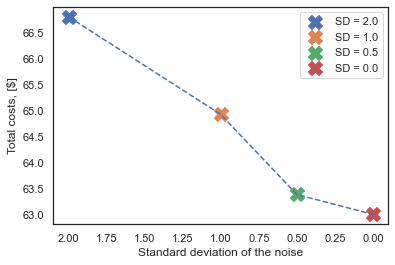
\includegraphics[width = 60mm]{TC_variance.png}
    \caption{Total cost of the agents w.r.t. variance of the noise in the forecasts}
    \label{fig: TC_variance}
    \vspace{-40pt}
\end{wrapfigure}

\begin{itemize}
    \item The effect of forecast purchases: agent $i$'s decision on the first stage depend on the forecast of $\Delta g_i$, so it is natural for agent $i$ to desire an increase in the quality of this forecast (Figure \ref{fig: TC_variance}).
    \begin{itemize}
        \item How does the buyer report the increase in the utility due to the better forecast? Is it possible to make this mechanism truthful? 
        
        \item Should we consider fixed payoff (or/and inclusion of reputation, dynamicity) for the forecast sellers to avoid this issue?
    \end{itemize}
    
    \item An indirect effect of the forecast market could appear from the forecast acquisition by some subset of agents on another agents. Concretely, can an improved forecast of agent $j$ (or a subset of agents $\subset \mathcal{N}$) improve the outcome for agent $i$?
    \begin{itemize}
        \item If so, will there be an incentive for agents to subsidize participation of all the agents in the forecast market? 
        
        \item What are the properties of the market?
    \end{itemize}
\end{itemize}

Below we describe a relevant blocks of the model.

\subsubsection{Forecast market}
We first adopt a model for the forecast market from \cite{raja} (Figure \ref{fig: data_market}). Let $i_C$ be a buyer \tcb{(in our case it is an agent participating in the forecast market)} who is interested in improving a forecast \tcb{(e.g., (i) forecasting algorithm (ii) weather forecast or (iii) a generation forecast for their renewable energy asset)}. For this purpose, the client enters the market by posting a forecasting task for an uncertain event $Y$, their own forecast report $r_c$ as a reference for improvement and an offer of a monetary value $\phi$ for per unit improvement.  Each seller $i \in I$ reports their forecast $r_i$ along with a wager $m_i >0$, which expresses their confidence on their forecast. We note that the client is also allowed to enter the market as a player with their own forecast report and wager. But as the client does not offer any improvement over their own reference forecast, in a truthful market setup, they receive no share from the resulting utility. However, the client can compete for a relative forecasting skill reward and also influence the resulting forecast. Finally, the market operator aggregates all the forecasts provided by the players, considering their wagers, and delivers the resulting report $\hat{r}(\mathbf{m}, \mathbf{r})$ to the client. 

After the occurrence of the event, i.e., the time interval for which the forecast is being elicited, the market operator observes the true outcome $\omega$ and evaluates the score $s(r_i, \omega)$ of each player $i \in I$, which shows how ``good'' was the forecast reported by player $i$. Furthermore, the operator also evaluates the utility allocated by the client for the forecast improvement $U(r_c, r, \omega, \phi)$ in monetary terms, which then has to be distributed among the players that have contributed to the improvement. \tcb{In order to design a reliable mechanism, we have to change this component of the payoff, as the buyers might not evaluate their utility increase prior to the market clearing due to the presence of the other agents. Building a mechanism will consist of several steps: (i) only skill-based part of the payoff (ii) fixed price based on reputation (or wager) of the seller. In order to include the latter, we can take several steps of increasing complexity again: (i) exogenous reputation scores (ii) endogenous reputation mechanism, updating the reputation after peer-to-peer market clearing.}

The mechanism design of this market model requires three main components: (i) an aggregation operator (to combine forecasts), (ii) a scoring rule, and (iii) a payoff allocation mechanism. 
\begin{itemize}
    \item {\it Aggregation operator:}  For each player $i \in I$, let $r_i$ be the forecast report in terms of probability distribution function and $R_i$ be the corresponding cumulative distribution function. Then, the average quantile forecast is given by $\hat{r}_{QA} = \sum_i \hat{m}_i R^{-1}_i$. 
    
    \item {\it Scoring rule:} For an event of interest $x$, let the probability density function reported by a player be $r$, and let $\omega$ be the event that actually occurred. Let $R$ denote the cumulative distribution. Then, the continuous ranked probability score is defined as 
    \begin{equation*}
        CRPS(R, \omega) := \int_{\infty}^{\infty} [R_r(x) - R_{\omega}(x)]^2 dx,
    \end{equation*}
    where $R_{\omega}(x) = 0$ if $x < \omega$ and $R_{\omega}(x) = 1$ otherwise.
    
    \item {\it Payoff allocation mechanism:} Payoff function is divided in two parts, one representing the allocation from the wager pool and another from the client’s allocated utility. The former evaluates the relative forecasting skill of a player, and the latter compensates for their contribution to an improvement of the client’s utility $U$.  Let the wager payoff of a player $i$ be 
    \begin{equation*}
        \Pi_i (\mathbf{r}, \mathbf{m}, \omega) := m_i \big(1 + s(r_i, \omega) - \frac{\sum_j s(r_j, \omega) m_j}{\sum_j m_j} \big).
    \end{equation*}
    An overall payoff is given as
    \begin{equation*}
        \hat{\Pi}_i := \Pi_i + \mathbbm{1}_{U >0} \Big( \frac{\tilde{s}(r_i, \omega) m_i}{\sum_j \tilde{s}(r_j, \omega) m_j} U \Big),
    \end{equation*}
    where $\tilde{s}(r_i, \omega):=\mathbbm{1}_{s(r_i, \omega) > s(r_c, \omega)} s(r_i, \omega)$.
\end{itemize}

\begin{figure}
    \centering
    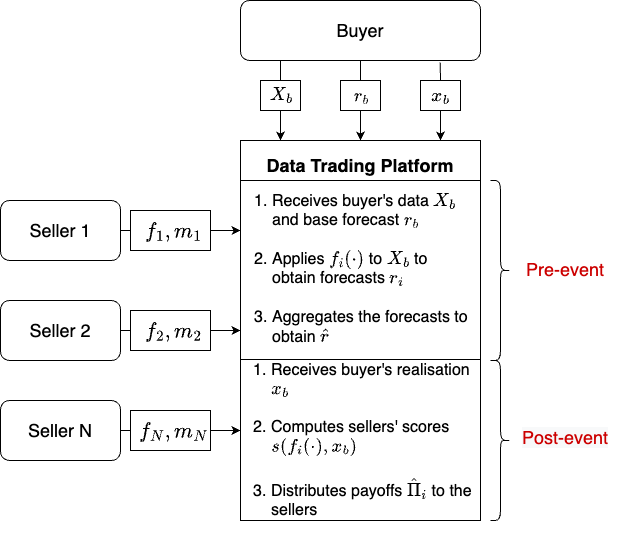
\includegraphics[width = 100mm]{data_market.png}
    \caption{Proposed data market scheme}
    \label{fig: data_market}
\end{figure}

%We are mainly interested in coupling this proposed model with the electricity market. The main connection point is $\phi$ or $U$ - the utility of the buyer that is later used for the payoffs. If we can evaluate the increase in the utility of the buyer caused by forecasts acquisition, then we can connect the two. Below, we consider several frameworks and discuss the challenges associated with them.



Some insights about the questions stated above can be obtained through numerical experiments. The code for the data market, one-agent electricity market and peer-to-peer electricity market (centralized solution) can be found at \cite{github}. In Appendix (section \ref{section: appendix}) I have put some additional extractions from the relevant papers.

\subsubsection{Numerical experiments}
In the numerical experiment I coupled the two markets, with 25 agents in the peer-to-peer market and 25 sellers on the forecast selling market. In order for the design of experiment to correspond to the one presented in Figure \ref{fig: data_market}, I took Pecan Street \cite{pecan_street} data consisting of 15-minutes intervals measuring appliances' consumption and renewable generation for 25 residential prosumers for one year. As a historical data $X_b$, each agent provides observations of RES-generation, from which the sellers build a distribution, subsequently used as a forecast $r_s$. An example of the forecast sold on the market is shown on Figure \ref{fig: res_dist}.  

\begin{wrapfigure}{r}{7cm}
    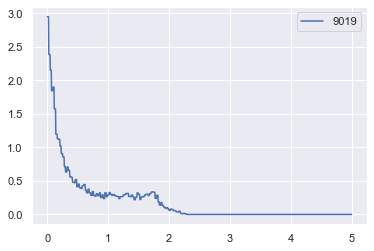
\includegraphics[width = 60mm]{res_dist.png}
    \caption{Example of the distribution used as a forecast}
    \label{fig: res_dist}
\end{wrapfigure}
Initially, each buyer of the forecast (an agent in the peer-to-peer market) uses as a base forecast a uniform distribution $U[0,7]$, which means that they are completely ignorant and do not have any information about their own generation. It was done in order to test the market coupling and to obtain some insights about its' properties. An actual generation $\Delta g_b$ (for each agent $b$) is a value sampled from the corresponding distribution. So, each agent on the peer-to-peer has a corresponding seller on the forecast market, who in turn has an access to an actual distribution of the renewable generation of this agent. This illustrates a situation, in which the sellers have better forecasts then the agents on the peer-to-peer market, thus making it profitable for the latter to purchase the forecasts from the former. 

First we considered the situation, in which there's only one agent purchasing the contract. We observed that it decreased real cost (cost computed using realization of $\Delta g_i)$ for the agent purchasing the forecast, while the costs of the other agents remained the same.  We used a following result to compute trading costs:
\begin{proposition}\label{proposition: trading costs}
    In the peer-to-peer market presented in \eqref{eq: two-stage initial formulation}, bilateral trading costs are equal to the day-ahead buying price $p^b_{da}$. The trading costs of agent $i$ are thus computed as $p^b_{da} \sum_{j \in \Gamma_i} q_{ij}$.
\end{proposition}
\begin{proof}
    Clearly, bilateral price $p^q_{ij}$ for peer-to-peer trading is bigger than $p^s_{da}$ and lower than $p^b_{da}$: $p^s_{da} \leq p^q_{ij} \leq p^b_{da}$ for each $i,j$. Denote $p^q_{ij} = p^b_{da} - \varepsilon$ for some $\varepsilon > 0$. Then, for any $\varepsilon > 0$, it's profitable for the agents to buy/sell energy. Taking $\varepsilon \rightarrow 0$, we conclude the proof.
\end{proof}

With trading costs computed as in Proposition \ref{proposition: trading costs}, we obtained a result, that any agent can improve only her outcome, given that she purchased a better forecast on the market, then her base one. As in one-shot game there's no mechanism for an agent to know in advance whether the acquired forecast is better than her base forecast, it's easy to obtain an example in which agent increases the cost after purchasing the forecast (e.g. taking truncated $\mathcal{N}(\Delta g_i, 1)$ as a base forecast). This can be overcome by proposing a dynamic model with reputation mechanism, that connects wager mechanism from \cite{raja} and the outcome of the peer-to-peer market. More precisely, we play repeated game depicted in Figure \ref{fig: data_market}, in which the wagers are decided by the platform and not by the forecast sellers. The wager update mechanism implemented by the platform should increment the wager of seller $i$ is $s(r_i, x_b) > s(r_b, x_b)$ and decrease it otherwise. 

What concerns one-shot game, it represents a variation of constrained newsvendor problem. Below we provide an initial analysis of the problem.

\subsubsection{KKT conditions}
First, we write a Lagrangian in a scenario-based framework
\begin{equation}
    \begin{aligned}
        \mathcal{L}_i &= p^b_{da} q^{da,b}_i - p^s_{da} q^{da, s}_i + \sum_{t \in T} p^t \big[ p^b_{rt} q^{rt,b}_{i,t} - p^s_{rt} q^{rt, s}_{i, t} \big] + \sum_{j \in \Gamma_i} \zeta_{ij} (q_{ij} + q_{ji}) + \sum_{j \in \Gamma_i} \xi_{ij} (q_{ij} - \kappa_{ij}) \\
        &+ \sum_{t \in T} \lambda^t_i (d_i - \Delta g_i - \sum_{j \in \Gamma_i} q_{ij} - q^{da,b}_i + q^{da,s}_{i,t} - q^{rt,b}_{i,t} + q^{rt,s}_i) - \mu^{da, b}_i q^{da, b}_i - \mu^{da,s}_i q^{da,s}_i - \mu^{rt,b}_{i,t} q^{rt,b}_{i.t} - \mu^{rt, s}_{i,t} q^{rt,s}_{i,t}
    \end{aligned}
\end{equation}

Then, first order stationarity conditions give:
\begin{align}
    \frac{\partial \mathcal{L}_i}{\partial q^{da, b}_i} &= p^b_{da} - \sum_{t \in T} \lambda^t_i - \mu^{da,b}_i = 0 \\
    \frac{\partial \mathcal{L}_i}{\partial q^{da, s}_i} &= -p^s_{da} + \sum_{t \in T} \lambda^t_i - \mu^{da,s}_i = 0 \\
    \frac{\partial \mathcal{L}_i}{\partial q_{ij}} &= \zeta_{ij} + \xi_{ij} - \sum_{t \in T} \lambda^t_i = 0 \\
    \frac{\partial \mathcal{L}_i}{\partial q^{rt, b}_{i,t}} &= p^t p^b_{rt} -  \lambda^t_i - \mu^{rt,b}_{i,t} = 0 \\
    \frac{\partial \mathcal{L}_i}{\partial q^{rt, s}_{i,t}} &= - p^t p^s_{rt} +  \lambda^t_i - \mu^{da,s}_{i,t} = 0 
\end{align}

From first two equations we get that $p^{b}_{da} - p^s_{da} = \mu^{da,b}_i + \mu^{da,s}_i > 0$, which (from complementarity conditions) means that we naturally have the (obvious) property that agent $i$ can not simultaneously buy and sell energy from the backup retailer (the same holds for a real-time market). Then, for the bilateral trading price we get that 
\begin{equation}
    \zeta_{ij} = p^b_{da} - \xi_{ij} - \mu^{da,b}_i = p^s_{da} - \xi_{ij} + \mu^{da,s}_i
\end{equation}

\subsubsection{Analysis of the cost}
In the end the total cost of agent $i$ can be expressed as a sum of first-stage cost, second-stage cost observed after realization of random variable $\Delta g_i$ and trading cost. First, note that the second stage decision is completely defined by the first-stage decision through the supply-demand balance constraint:
\begin{equation}
    q^{rt, b}_{i, t} - q^{rt, s}_{i,t} = \overbrace{d_i - \Delta g^t_i - q^{da,b}_i + q^{da,s}_i - \sum_{j \in \Gamma_i} q_{ij}}^{s^t_i}
\end{equation}
Note that $q^{rt, b}_{i, t} \cdot q^{rt, s}_{i,t} = 0$, thus we can rewrite the equation above as 
\begin{equation}
    q^{rt, b}_{i, t} = s^t_i \quad  if \quad s^t_i \geq 0 \qquad else \qquad q^{rt, s}_{i, t} = -s^t_i
\end{equation} 
Then, we can insert it into the total cost function 
\begin{equation}
    \Pi_i : = p^b_{da} q^{da,b}_i - p^s_{da} q^{da,s}_i + \sum_{t \in T} p^t \big[ p^b_{rt} s^t_i \cdot \mathbb{I}_{s^t_i \geq 0} + p^s_{rt} s^t_i \cdot \mathbb{I}_{s^t_i \leq 0} \big] + p^b_{da} \sum_{j \in \Gamma_i} q_{ij}
\end{equation}
Let's expand the second-stage costs:
\begin{equation}
    \sum_{t \in T} p^t \big[ p^b_{rt} [d_i - \Delta g^t_i - q^{da,b}_i + q^{da,s}_i - \sum_{j \in \Gamma_i} q_{ij}] \cdot \mathbb{I}_{s^t_i \geq 0} + p^s_{rt} [d_i - \Delta g^t_i - q^{da,b}_i + q^{da,s}_i - \sum_{j \in \Gamma_i} q_{ij}] \cdot \mathbb{I}_{s^t_i \leq 0} \big]
\end{equation}

For the sake of analytical derivation, we write below $f(\Delta g_i)$ as a density function instead of $p^t$ (we will later return to discretized form):
\begin{equation*}
    \begin{aligned}
        \Pi^{second}_i &= -p^b_{rt}\int_{0}^{\infty} f(\Delta g_i) \Delta g_i \cdot \mathbb{I}_{s^t_i \geq 0} d \Delta g_i + p^b_{rt}\int_{0}^{\infty} f(\Delta g_i) [d_i - q^{da,b}_i + q^{da,s}_i - \sum_{j \in \Gamma_i} q_{ij}] \cdot \mathbb{I}_{s^t_i \geq 0} d \Delta g_i  \\
        &-p^s_{rt}\int_{0}^{\infty} f(\Delta g_i) \Delta g_i \cdot \mathbb{I}_{s^t_i \leq 0} d \Delta g_i  + p^s_{rt}\int_{0}^{\infty} f(\Delta g_i) [d_i - q^{da,b}_i + q^{da,s}_i - \sum_{j \in \Gamma_i} q_{ij}] \cdot \mathbb{I}_{s^t_i \leq 0}  d \Delta g_i = \\
        &= - p^b_{rt} \int_0^{d_i - q^{da,b}_i + q^{da,s}_i - \sum_{j \in \Gamma_i} q_{ij}} \Delta g_i f(\Delta g_i) d \Delta g_i  + p^b_{rt}(d_i - q^{da,b}_i + q^{da,s}_i - \sum_{j \in \Gamma_i} q_{ij}) \mathbb{P}(\Delta g_i \leq d_i - q^{da,b}_i + q^{da,s}_i - \sum_{j \in \Gamma_i} q_{ij})\\
        & -p^s_{rt} \int_{d_i - q^{da,b}_i + q^{da,s}_i - \sum_{j \in \Gamma_i} q_{ij}}^{\infty} \Delta g_i f(\Delta g_i) d \Delta g_i  + p^s_{rt} (d_i - q^{da,b}_i + q^{da,s}_i - \sum_{j \in \Gamma_i} q_{ij}) \mathbb{P}(\Delta g_i \geq d_i - q^{da,b}_i + q^{da,s}_i - \sum_{j \in \Gamma_i} q_{ij})
    \end{aligned}
\end{equation*}
Denote residual after first-stage decisions as $r_i:=d_i - q^{da,b}_i + q^{da,s}_i - \sum_{j \in \Gamma_i} q_{ij}$ and note that it is obviously non-negative. Then, second stage costs can be rewritten as 
\begin{equation}
    \begin{aligned}
        \Pi^{second}_i &= -p^b_{rt} \int_{0}^{r_i} \Delta g_i f(\Delta g_i) d \Delta g_i + p^b_{rt} r_i \mathbb{P} (\Delta g_i \leq r_i) - p^s_{rt} \int_{r_i}^{\infty} \Delta g_i f(\Delta g_i) d \Delta g_i  + p^s_{rt} r_i \mathbb{P} (\Delta g_i \geq r_i)\\
        &= p^b_{rt} r_i F (r_i) + p^s_{rt} r_i (1 -  F(r_i)) - p^b_{rt} \int_{0}^{r_i} \Delta g_i f(\Delta g_i) d \Delta g_i - p^s_{rt} \int_{r_i}^{\infty} \Delta g_i f(\Delta g_i) d \Delta g_i
    \end{aligned}
\end{equation}

\begin{thebibliography}{}

\bibitem{raja} A. A. Raja, P. Pinson, J. Kazempour, S. Grammatico, ``A Market for Trading Forecasts: A Wagering Mechanism''. arXiv preprint arXiv:2205.02668, 2022.

\bibitem{moret} F. Moret, P. Pinson, and A. Papakonstantinou, ``Heterogeneous risk preferences in community-based electricity markets'', {\it European Journal of Operational Research}, vol. 287, no. 1, pp. 36-48, 2020. 

\bibitem{perakis} G. Perakis, G. Roels, ``Regret in the Newsvendor Model with Partial Information'', {\it Operations Research}, 56 188-203, 2008.

\bibitem{nair} J. Nair, S. Adlakha, A. Wierman, ``Energy Procurement Strategies in the Presence of Intermittent Sources'', {\it ACM SIGMETRICS Performance Evaluation Review}, 42, 2014

\bibitem{github} \url{https://github.com/ishilov/data_market}

\bibitem[Pecan Street (2022)]{pecan_street} Pecan Street Dataport. [online] Available: https://dataport.pecanstreet.org/.

\end{thebibliography}

\newpage
\section{Appendix}\label{section: appendix}
For a motivating example consider the newsvendor problem with back order and stock holding costs from \cite{perakis}. Consider a make-to-stock firm that needs to determine its order quantity $y$ before the selling season, without knowing the demand. The demand $D$ is random and has a cumulative distribution function (c.d.f.) $F$. Assume linear costs and denote by $r$ the unit selling price, $s$ the unit salvage price, $l$ the loss of goodwill cost per unit of unsatisfied demand, and $c$ the unit cost. 

\begin{equation*}
    \max_{y \geq 0 } \Pi_F(y) := r \mathbb{E}_F \min\{y,D\} + s \mathbb{E}_F [y - D]^+ - l \mathbb{E}_F [D-y]^+ - c y
\end{equation*}
The optimal order quantity is the smallest $y$ such that $F(y) \geq 1 - \beta$, where $\beta := (c - s) / (r + l - s)$. If the demand distribution is continuous, the optimality condition simplifies to $F(y) = 1 - \beta$. In \cite{perakis}, authors consider different situations of the a priori information available to the newsvendor (mean, median, range etc.). In our case it is a bit different, if we want to build a forecast market: the possible data to provide is the better prediction of the p.d.f $f$ of the distribution \cite{raja}, e.g., for $D$ we can consider possible values $\{1, 2, 3, 4, 5 \}$ with provided forecasts looking like $\{0.1, 0.1, 0.6, 0.1, 0.1\}$ , $\{0, 0.2, 0.6, 0.2, 0\}$ and $\{0.2, 0, 0.6, 0, 0.2\}$. Then, the newsvendor can choose which forecast to purchase (or how to combine them, see \cite{raja}) and the payment can be made based on the relative improvement to the base forecast of the newsvendor.

\begin{figure}[h]
    \centering
    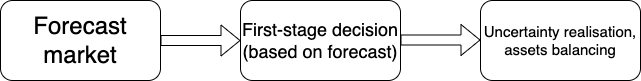
\includegraphics[width = 100mm]{high_level_steps.png}
    \caption{High-level representation }
    \label{fig:1}
\end{figure}

If we assume all the information (in this case it is $r, s, l, c$) is known by forecast sellers, then it is easy to evaluate the relative gain acquired because of the forecast, which then can be used to make payments.



\subsection{Electricity market}
\subsubsection{One-agent model}
Starting point in our consideration of the coupling data market and electricity market could be to consider a one-agent formulation of the latter. For our needs, we can adapt a formulation from \cite{nair}, which represents a variant of the newsvendor problem. 

Assume the demand $d$ to be known ahead of time. In \cite{nair} authors consider a utility company with long term contracts for uncertain, intermittent, renewable energy. Given such a long term contract, the utility company participates in a three tiered market for conventional generation consisting of: 
\begin{itemize}
    \item a long term market, in which a purchase commitment is made at time $-T_{lt}$ and the price of energy is $p_{lt}$
    
    \item an intermediate market (typically day ahead), in which a purchase commitment is made at time $-T_{in}$ and the price of energy is $p_{in}$
    
    \item a real time market, in which purchase commitment is made at time $t = 0$ and the price of energy is $p_{rt}$
\end{itemize}
with $-T_{lt} < -T_{in} < 0$ and $0 < p_{lt} < p_{in} < p_{rt}$.

Let $\omega$ denote the actual wind energy that is available at time $t = 0$, that  the utility company comes to know at time $t = 0$. Let $\hat{\omega}_{lt}$ and $\hat{\omega}_{in}$ denote respectively the
forecasts of $\omega$ available at the time of the long term market (i.e., at $t = -T_{lt}$) and the intermediate market (i.e., at $t = -T_{in}$). Formally,  assume that
\begin{equation*}
    \hat{\omega}_{in} = \hat{\omega}_{lt} - \mathcal{E}_1, \quad \text{and}  \quad \omega = \hat{\omega}_{in} - \mathcal{E}_2 
\end{equation*}
where $\mathcal{E}_1$ and $\mathcal{E}_2$ are zero mean independent random variables. 

Let $q_{lt}(\hat{\omega}_{lt})$ denote the quantity of conventional generation procured in the long term market, given the long term wind estimate $\hat{\omega}_{lt}$. Similarly, let $q_{in}(\hat{\omega}_{in}, q_{lt})$ denote the quantity of conventional generation procured in the intermediate market, given the corresponding wind estimate $\hat{\omega}_{in}$ and $q_{lt}$ (the quantity procured already). Finally, let $q_{rt}(\omega, q_{lt} + q_{in})$ denote the the quantity of conventional generation procured in the real time market, which depends on the realized wind $\omega$, and the quantity procured already, i.e., $q_{lt} + q_{in}$. For notational convenience we can simply write $q_{lt}, q_{in}, q_{rt}$. Then, we can write the optimal procurement problem as follows:
\begin{align*}
    \min_{q_{lt}, q_{in}, q_{rt}} &\mathbb{E}[p_{lt} q_{lt} + p_{in} q_{in} + p_{rt} q_{rt}]\\
    s.t.\quad & q_{lt} \geq 0, q_{in} \geq 0, q_{rt} \geq 0\\
    & q_{lt} + q_{in} + q_{rt} + \omega \geq d
\end{align*}

Authors then provide a result that characterizes the optimal procurement strategy for a utility company in a three tiered market:
\begin{theorem}
    The optimal procurement strategy for the utility company in the three tiered market scenario is:
    \begin{align*}
        q^{\ast}_{lt} &= [d - \hat{\omega}_{lt} + r_{lt}]_+ \\
        q^{\ast}_{in} &= [d - \hat{\omega}_{in} - q_{lt} + r_{in}]_+ \\
        q^{\ast}_{rt} &= [d - \omega - (q_{lt} + q_{in})]_+,
    \end{align*}
    where (with $\bar{F}_X(x) = P(X > x)$)
    \begin{equation*}
        r_{in} = \bar{F}^{-1}_{\mathcal{E}_2} \big( \frac{p_{in}}{p_{rt}} \big),
    \end{equation*}
    and $r_{lt}$ is the unique solution of
    \begin{equation*}
        h(r) := p_{lt} - p_{in} \bar{F}_{\mathcal{E}_1} (r - r_{in}) - p_{rt} P(\mathcal{E}_1 + \mathcal{E}_2 > r, \mathcal{E}_1 \leq r - r_{in}) = 0
    \end{equation*}
\end{theorem}
A key feature of this result is that the structure of the the optimal procurement strategy gives a natural interpretation to $r_{lt}$ and $r_{in}$ as reserve levels. Specifically, at the time of purchase in the long term market, $d - \hat{\omega}_{lt}$ can be interpreted as an estimate of the conventional procurement that is required to meet the demand. Then $r_{lt}$ is the additional 'reserve' purchased by the utility to balance the current wind uncertainty and the higher cost of conventional energy in subsequent markets. The reserve $r_{in}$ has a similar interpretation.

\subsubsection{Connection with the data market}
Clearly, the resulting expected cost of utility company here is $\Pi^{\ast}_c := \mathbb{E}[p_{lt} q^{\ast}_{lt} + p_{in} q^{\ast}_{in} + p_{rt} q^{\ast}_{rt}]$. Let's denote the forecasts introduced above as $r_c := \mathcal{E}_{1,2}$. If utility company has an access to another forecasts (say $\hat{r} := \hat{\mathcal{E}}_{1,2}$), then the resulting expected costs would be $\hat{\Pi}^{\ast}_c := \mathbb{E}[p_{lt} \hat{q}^{\ast}_{lt} + p_{in} \hat{q}^{\ast}_{in} + p_{rt} \hat{q}^{\ast}_{rt}]$, which will allow us to write a respective utility improvement as $U = \Pi^{\ast}_c - \hat{\Pi}^{\ast}_c$. We can reasonably assume that the prices $p_{lt}, p_{in}, p_{rt}$ are known to all the participants of the market (both forecast sellers and MO), thus, allowing them to calculate this difference by themselves and subsequently use it in the payoff allocation step. It follows, that the coupling of these two models is straightforward.

\subsubsection{Peer-to-peer trading in real-time market}
In this formulation, agents decide on the bilateral trades in the real-time market. It means that the decision variables of the second stage are $q^{rt,b}_i, q^{rt,s}_i, \mathbf{q}_i$. Then, if we use scenario-based approach with a set of scenarios $\Omega$, we write electricity market formulation as follows:
\begin{equation}\label{eq: two-stage second formulation}
    \begin{aligned}
        \min_{q^{da}_i, q^{rt}_i, \mathbf{q}_{i}} \quad &  \overbrace{p^b_{da} q^{da,b}_i - p^s_{da} q^{da,s}_i}^{1^{st} \text{ stage costs }} + \mathbb{E}_{\omega}\Big[\,\overbrace{p^b_{rt} q^{rt, b}_i - p^s_{rt} q^{rt,s}_i}^{2^{nd} \text{ stage costs }} \,\Big] \\
        s.t. \quad & q^{da,b}_i \geq 0, q^{da,s}_i \geq 0, q^{rt,b}_i \geq 0, q^{rt,s}_i \geq 0\\
        & q^{\omega}_{ij} + q^{\omega}_{ji} = 0, \qquad \forall j \in \Gamma_i, \forall \omega \in \Omega\\
        & q^{\omega}_{ij} \leq \kappa_{ij}, \qquad \forall j \in \Gamma_i, \forall \omega \in \Omega \\
        & d_i = \Delta g_i + \sum_{j \in \Gamma_i} q^{\omega}_{ij} + q^{da,b}_i - q^{da,s}_i + q^{rt,b}_i - q^{rt,s}_i\\
    \end{aligned}
\end{equation}
The difficulties in this formulation come form the need to anticipate trading decisions $q^{\omega}_{ji}, j \in \Gamma_i$ of the other agents in the market. Thus, in this formulation, agents need to have a forecast (a belief) about other agents' random generation, which motivates us to propose a forecast market, where agents can sell forecasts about their own future generation (we assume that agent $i$ has a most accurate forecast of her own production $\Delta g_i$). This formulation, even in its simple form as in \eqref{eq: two-stage second formulation} is more complicated and poses non-trivial questions:
\begin{itemize}
    \item What are the advantages to employ inter-agent trading on the second-stage market? A guess could be that it brings more accurate trading decisions, as we allocate bigger volume of energy traded to a real-time market, shifting it from the first stage, thus allowing to reduce balancing costs induced by backup retailer.
    \begin{itemize}
        \item The first step would be to verify this claim numerically, using Monte-Carlo or an approximation.
    \end{itemize}
    
    \item How to define coupling constraints $q^{\omega}_{ij} + q^{\omega}_{ji} = 0$ w.r.t. randomness on the first stage? On the first-stage market, when agents anticipate other agents' decisions, they need to have an access to an information about other agents' forecasts. 
    \begin{itemize}
        \item In order to accurately make decisions on the first stage, agents need to know (in the best case) a closed form expression for $q^{\omega}_{ji}(\Delta \mathbf{g}_i)$ or some approximate solution $\tilde{q}^{\omega}_{ji}(\Delta \mathbf{g}_i)$ which would depend on $\Delta \mathbf{g}_i$ - a vector of other agents' forecasts. 
        
        \item In this case, decision quality on the first stage will depend not only on agent $i$'s quality of the forecast (beliefs) about other agents' distribution, but also on the quality of approximation $\tilde{q}^{\omega}_{ji}$.
        
        \item Even with an access to high quality forecasts of the other agents, we need to account for correlation between agents in their distribution of $\Delta g_i$.
    \end{itemize}
    
    \item In view of above points, forecast market should be adjusted accordingly. 
    \begin{itemize}
        \item First formulation could be to employ the model proposed in \cite{raja} on an agent-to-agent basis, in which we omit the {\it relative forecasting skill} part of the payoff. It means that agent $i$ chooses to purchase a forecast from agent $j$ about $\Delta g_j$, thus leaving only one seller for a forecasting task. 
        
        \item Evaluation of the forecast quality is a complicated task in an absence of market operator. We still might have a platform that verifies relative utility increase due to the forecast purchase, or we should employ other mechanisms.
    \end{itemize}
\end{itemize}

\end{document}
